

\section{Introduction%
  \label{introduction}%
}


\subsection{An overview of the ScopeSim environment%
  \label{an-overview-of-the-scopesim-environment}%
}

ScopeSim is a modular and flexible suite of python packages that enable (almost) any astronomical optical (observatory/telescope/instrument) system to be simulated.

The suite of packages can be used by a wide audience for a variety of purposes; from the astronomer interested in simulating reduced observational data, to a pipeline developer needing raw calibration data for testing the pipeline.

\begin{figure}
\noindent\makebox[\linewidth][c]{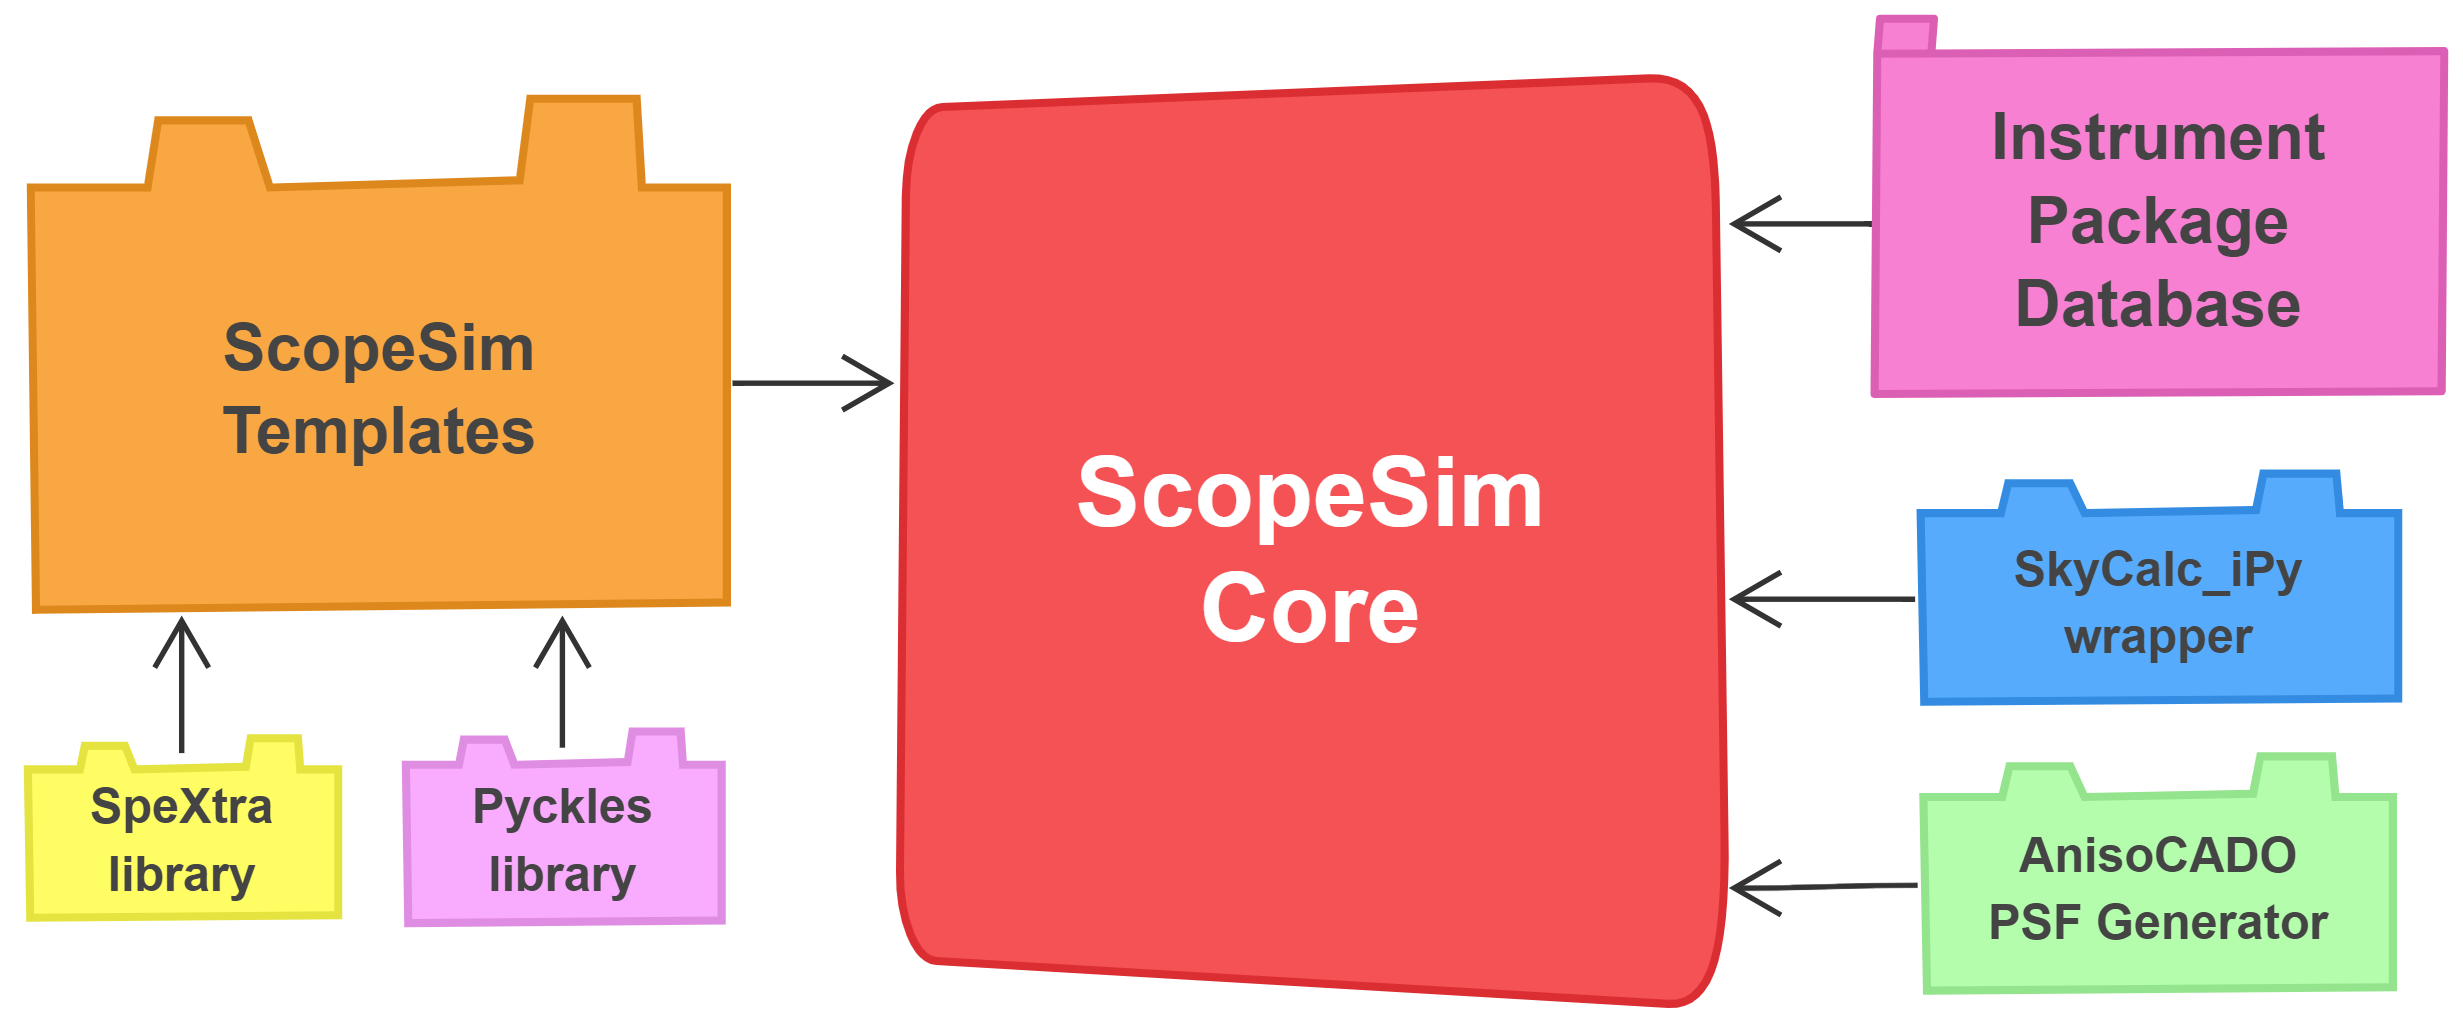
\includegraphics[scale=0.3]{images/scopesim_environment_overview.png}}\phantomsection\label{fig-scopesim-environment}
\caption{The packages belonging to the ScopeSim environment.}
\end{figure}

ScopeSim achieves this level of flexibility by adhering to strict interfaces between the package, e.g: the ScopeSim engine package is completely instrument and object agnostic.
All information and data relating to any specific optical configuration is kept exclusively in the instrument packages hosted in the instrument reference database (IRDB).
Similarily, the engine has no clue about what it is observing until run-time.
The description of the on-sky source is keep exclusively within the target \texttt{templates} package (see \texttt{scopesim\_templates}).

The core of the ScopeSim environment are the three packages:

\begin{itemize}
\item \texttt{ScopeSim}: the simulation engine

\item \texttt{ScopeSim\_templates}: descriptions of the on-sky sources

\item \texttt{IRDB}: the instrument reference database.
\end{itemize}

In addition to the core package, there are several support packages:

\begin{itemize}
\item \texttt{AnisoCADO}: simulates SCAO PSFs for the ELT

\item \texttt{SkyCalc\_ipy}: queries the ESO skycalc service for atmospheric spectral curves

\item \texttt{SpeXtra}: provides easy access to many well-known spectral libraries

\item \texttt{Pyckles}: a light-weight wrapper for the Pickles (1998) and Brown (2010) catalogues.
\end{itemize}

Each of these packages will be discussed in detail in the following sections.


\subsection{Document Scope%
  \label{document-scope}%
}

This document is not intended to be a comprehensive description of the ScopeSim environment. Rather is aims to introduce the reader to the elements that make up ScopeSim and directs the reader towards the online documentation for each of the packages, should the reader wish to dive deeper into the material.


\subsection{Rationale for the ScopeSim environment%
  \label{rationale-for-the-scopesim-environment}%
}

Until now most instrument consortia have developed their own simulators.
The general argument is that every new instrument is sufficiently different from anything that has been previously developed, that it would make no sense to adapt already existing code.
This statement is true to some extent.
Every new instrument must differ in some way from all existing instruments in order for it to be useful to the astronomical community.
However when looked at from a global perspective, every optical system is comprised primarily of elements common to all other systems.
Atmospheric emission, mirror reflectivities, filter transmission curves, point spread functions, read-out noise, detector linearity, hot pixels, are just a few of the effects and artifacts that every astronomical optical system contains.
Furthermore, while the amplitude and shape of each effect differs between optical systems, there are still commonalities in the way each effect can be described programmatically.

ScopeSim's main goal is to provide a framework for modelling (almost) any astronomical optical system by taking advantage of all these commonalities.
What astropy has done for python landscape in astronomy, ScopeSim aims to do for the instrument simulator landscape.


\subsection{Community involvement%
  \label{community-involvement}%
}

The scopesim environment has been developed as an open source project so that it is possible for others in the astronomical community to be involved in the expansion of both core and perifery functionality.
The interface of both the \texttt{Effect} and \texttt{Source} objects was kept as minimalistic in order to keep the barrier to entry as low as possible.

For the \texttt{ScopeSim\_templates} package we encourage the submission of both basic and detailed custom \texttt{Source} objects for any astronomical source.
The package is designed in such a way as to be highly scalable to accommodate descriptions of the myriad of astronomical objects.

For users who need custom \texttt{Effect} objects for their optical model, there is the possibility of adding \textquotedbl{}plug-in\textquotedbl{} \texttt{Effect} objects at run time.
We however encourage anyone who has made these custom \texttt{Effects} to submit a pull request to the ScopeSim github page, so that we can include these \texttt{Effects} in the next major release.


\subsection{Documentation and code bases%
  \label{documentation-and-code-bases}%
}

\setlength{\DUtablewidth}{\linewidth}
\begin{longtable}[c]{|p{0.315\DUtablewidth}|p{0.315\DUtablewidth}|p{0.315\DUtablewidth}|}
\caption{Links to the open source doumentation and code bases}\\
\hline

Package
 & 
Documentation
 & 
Code base
 \\
\hline

ScopeSim
 & 
\url{https://scopesim.readthedocs.io/}
 & 
\url{https://github.io/astronomyk/scopesim}
 \\
\hline

ScopeSim\_templates
 & 
\url{https://scopesim-templates.readthedocs.io/}
 & 
\url{https://github.com/astronomyk/ScopeSim_templates}
 \\
\hline

IRDB
 & 
\url{https://irdb.readthedocs.io/en/latest/}
 & 
\url{https://github.com/astronomyk/IRDB}
 \\
\hline

AnisoCADO
 & 
\url{https://anisocado.readthedocs.io/}
 & 
\url{https://github.com/astronomyk/AnisoCADO}
 \\
\hline

SkyCalc\_ipy
 & 
\url{https://skycalc-ipy.readthedocs.io/en/latest/}
 & 
\url{https://github.com/astronomyk/SkyCalc_iPy}
 \\
\hline

SpeXtra
 & 
\url{https://spextra.readthedocs.io/en/latest/}
 & 
\url{https://github.com/miguelverdugo/speXtra}
 \\
\hline

Pyckles
 & 
\url{https://pyckles.readthedocs.io/en/latest/}
 & 
\url{https://github.com/astronomyk/Pyckles}
 \\
\hline
\end{longtable}
\label{tbl-list-of-packages}
